\documentclass[a4paper,english,12pt,bibliography=totoc]{scrreprt}

\usepackage[T1]{fontenc} %immer
\usepackage[utf8]{inputenc} %am
\usepackage{babel} %Anfang

\usepackage{enumitem} %Aufzählungen verändern

%Gleichungen verwenden
\usepackage{newtxtext}
\usepackage{amsmath}
\usepackage{amssymb}
\usepackage{mathptmx}
%\usepackage{txfonts}

\usepackage{listings}% code blocks
\usepackage[most]{tcolorbox}

%Querverweise
\usepackage{varioref} %immer
\usepackage{hyperref} %in dieser
\usepackage{cleveref} %Reihenfolge

\usepackage{booktabs} %schönere Tabellen
\usepackage{siunitx} %SI-Einheiten
\usepackage{tabularx} %Tabellen mit flexiblen Spalten	

\usepackage{graphicx} %Grafiken verwenden

\usepackage[backend=biber,style=numeric]{biblatex}
\addbibresource{main.bib} 

\usepackage{lipsum} %Blindtext
\usepackage{subcaption}
\usepackage{afterpage}
\usepackage[headsepline]{scrlayer-scrpage} %Paket für Kopfzeilen
\usepackage{afterpage}
\usepackage{float}
\automark[subsection]{section}

\pagestyle{scrheadings}
\ihead{} % oben links
\chead{\leftmark} % oben Mitte
\ohead{} % oben rechts
\cfoot{\pagemark} % unten Mitte
\automark[section]{section} % Modified line

% Zu volle hboxen korrigieren
\tolerance 1414
\hbadness 1414
\emergencystretch 1.5em
\hfuzz 0.3pt
\widowpenalty=10000
\vfuzz \hfuzz
\raggedbottom

%Informationen über das Dokument
\date{\today}


\begin{document}


\begin{titlepage}
	\centering
	
\includegraphics[width=0.8\textwidth]{logo_uulm_sw}
	
	\vspace{1cm}
	\LARGE Laboratory Module for Master Programs
	\Huge \textbf{Biophysics Lab Course}
	
	\vspace{1cm}
	\Large Experiment:

	\Huge \textbf{Stopped flow kinetics}
	
	\vspace{15mm}
	\Large Performed on 
	
	\vspace{5mm}
	\LARGE Group 8
	
	\vspace{1cm}
	\Large
	\begin{tabular}{rcl}
	\textbf{Haiyang Zhang} & and & \textbf{Nicolae Turcan}\\
	\href{mailto:student.1@uni-ulm.de}{haiyang.zhang@uni-ulm.de} & & \href{mailto:student.2@uni-ulm.de}{nicolae.turcan@uni-ulm.de}
	\end{tabular}
	
	\vspace{7mm}
	Supervisor: Thomas Vomhof
	
	\vfill
	\begin{tabular}{p{50mm}@{\hspace{5cm}}p{50mm}}
	\hrulefill & \hrulefill \\
	%\centering Haiyang Zhang  & \centering Nicolae Turcan
	\end{tabular}
	
	\vspace{5mm}
	\normalsize \raggedright
	We hereby confirm that we have elaborated the present work independently and have detailed knowledge of the entire contents.
\end{titlepage}



\tableofcontents

\chapter{Introduction}
\label{cha:Introduction}


%A Brief introduction to the protein folding and unfolding landscapes
Protein folding is the process by which a polypeptide sequence acquires its biologically functional three-dimensional structure. This process is driven by various intra-molecular interactions and results in a stable, lower-energy conformation. Understanding protein folding through the lens of energy landscapes ( see Figure 1.1) helps us to understand the complex nature of protein dynamics and stability, providing insights into how proteins attain their functional conformations and how misfolded proteins, called prions, can cause diseases like Bovine Spongiform Encephalopathy.

\begin{figure}[H]
    \centering
    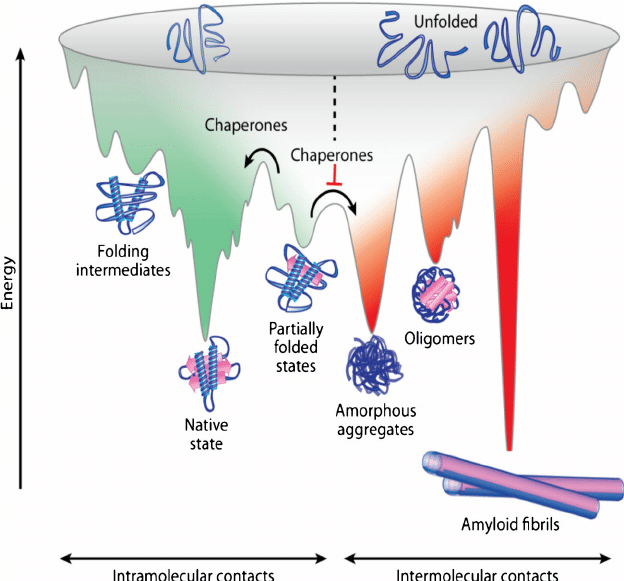
\includegraphics[width=0.5\linewidth]{Energy-landscape-of-protein-folding-and-misfolding-From-the-unfolded-state-toward-the.png}
    \caption{The Free energy landscape of a protein displaying possible conformations and Prion advantage \cite{muntau_innovative_2014}}
    \label{fig:enter-label}
\end{figure}

%Why protein folding is favorable entropically, why water takes more conformational states as a result, and how changing pH disfavors this.
Protein folding might seem counterintuitive regarding entropy since it reduces the number of possible states for the protein. However, the overall entropy change includes contributions from both the protein and the surrounding water. In the unfolded state, hydrophobic residues are exposed to water, forcing water molecules to arrange themselves in an ordered shell, decreasing their entropy. When the protein folds, these hydrophobic residues are buried, allowing water molecules to be more disordered and increasing their entropy. Thus, the increase in water entropy compensates greatly for the decrease in protein entropy, resulting in a favorable overall entropy change.\\

At very low or high pH values, proteins can denature, losing their three-dimensional structure. the reason is that extreme pH levels disrupt non-covalent interactions, such as hydrogen bonds, ionic bonds (such as those in Figure 1.4), and hydrophobic interactions, which are crucial for maintaining protein stability.\\

% How does stopped flow kinetics enable us to measure the folding/unfolding rate? Why turbulent is necessary flow?
Stopped-flow kinetics allows the measurement of protein folding and unfolding rates by rapidly mixing reactants and monitoring the reaction in real-time. Turbulent flow is essential in this technique to ensure rapid and homogeneous mixing of the reactants, which is necessary for initiating the reaction uniformly and maximizing the amount of time in which we can observe the rate of change during the linear phase. This enables accurate and reproducible measurements of the fast kinetic processes involved in protein folding and unfolding.\\

% Fluorescence of Tryptophan for the high Quantum Yield hydrophobic nature, is sensitive to the environment
Tryptophan is an excellent fluorophore for stopped-flow kinetics due to its strong intrinsic fluorescence, which allows it to naturally emit light when excited by UV light without external labeling. It has a high quantum yield, meaning it efficiently converts absorbed light into emitted fluorescence, resulting in strong and detectable signals.
\begin{figure}[H]
    \centering
    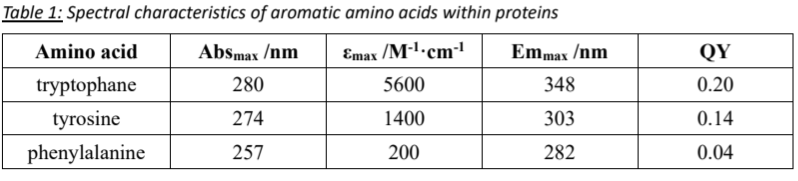
\includegraphics[width=0.9\linewidth]{tryptophanQY.png}
    \caption{A Table displaying the greater Quantum Yield of Tryptophan compared to other aromatic aminoacids \cite{BiophysicsLabCourse}}
\end{figure}
Its fluorescence is highly sensitive to the local environment, making it a valuable probe for monitoring protein folding and unfolding. Tryptophan emits at around 350 nm, a distinct wavelength that minimizes interference from other aromatic amino acids. Additionally, its fluorescence intensity and wavelength can vary significantly if the Tryptophan is buried in the core of the protein, shielded from interaction with water, or if is on the surface of the protein .

\begin{figure}[H]
    \centering
    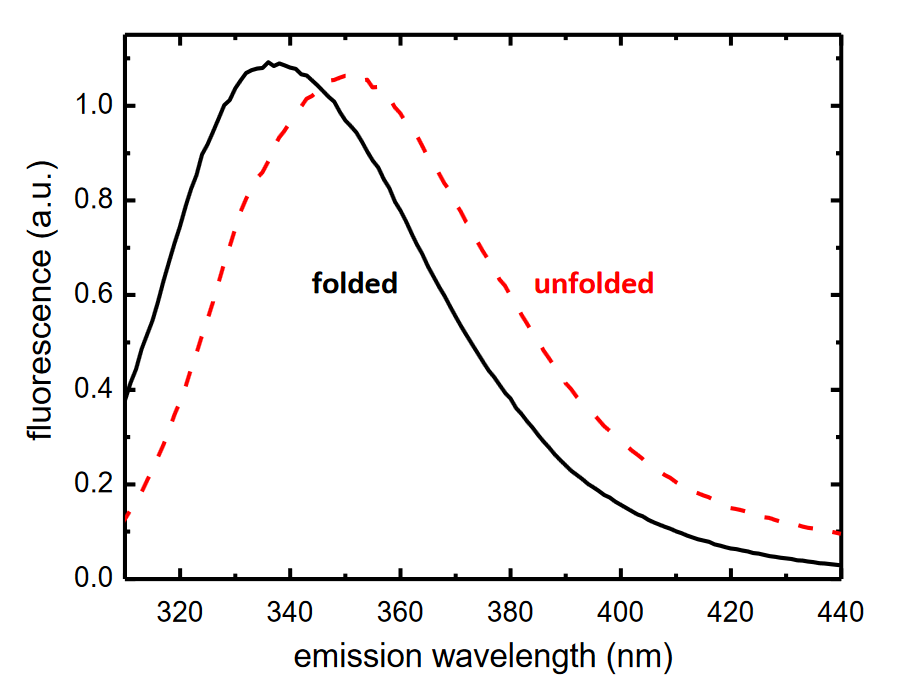
\includegraphics[width=0.5\linewidth]{tryptophan.png}
    \caption{Tryptophan Emission Spectra under solvent accessible/ inaccessible conditions \cite{BiophysicsLabCourse}}
\end{figure}

%Figure showing that 4 tryptophans are on the inside of the protein and unfolding puts them on the outside( shifting the emission spectrum )
The figure shows a protein structure rendered with Pymol \cite{pymol} in gray, highlighting its secondary elements such as helices and loops. Two chlorine ions are depicted as lime spheres. Several tryptophan residues are marked in magenta, emphasizing their locations and orientations within the protein structure. These are the tryptophan residues used as fluorescent probes to study the conformational changes.

\begin{figure}
    \centering
    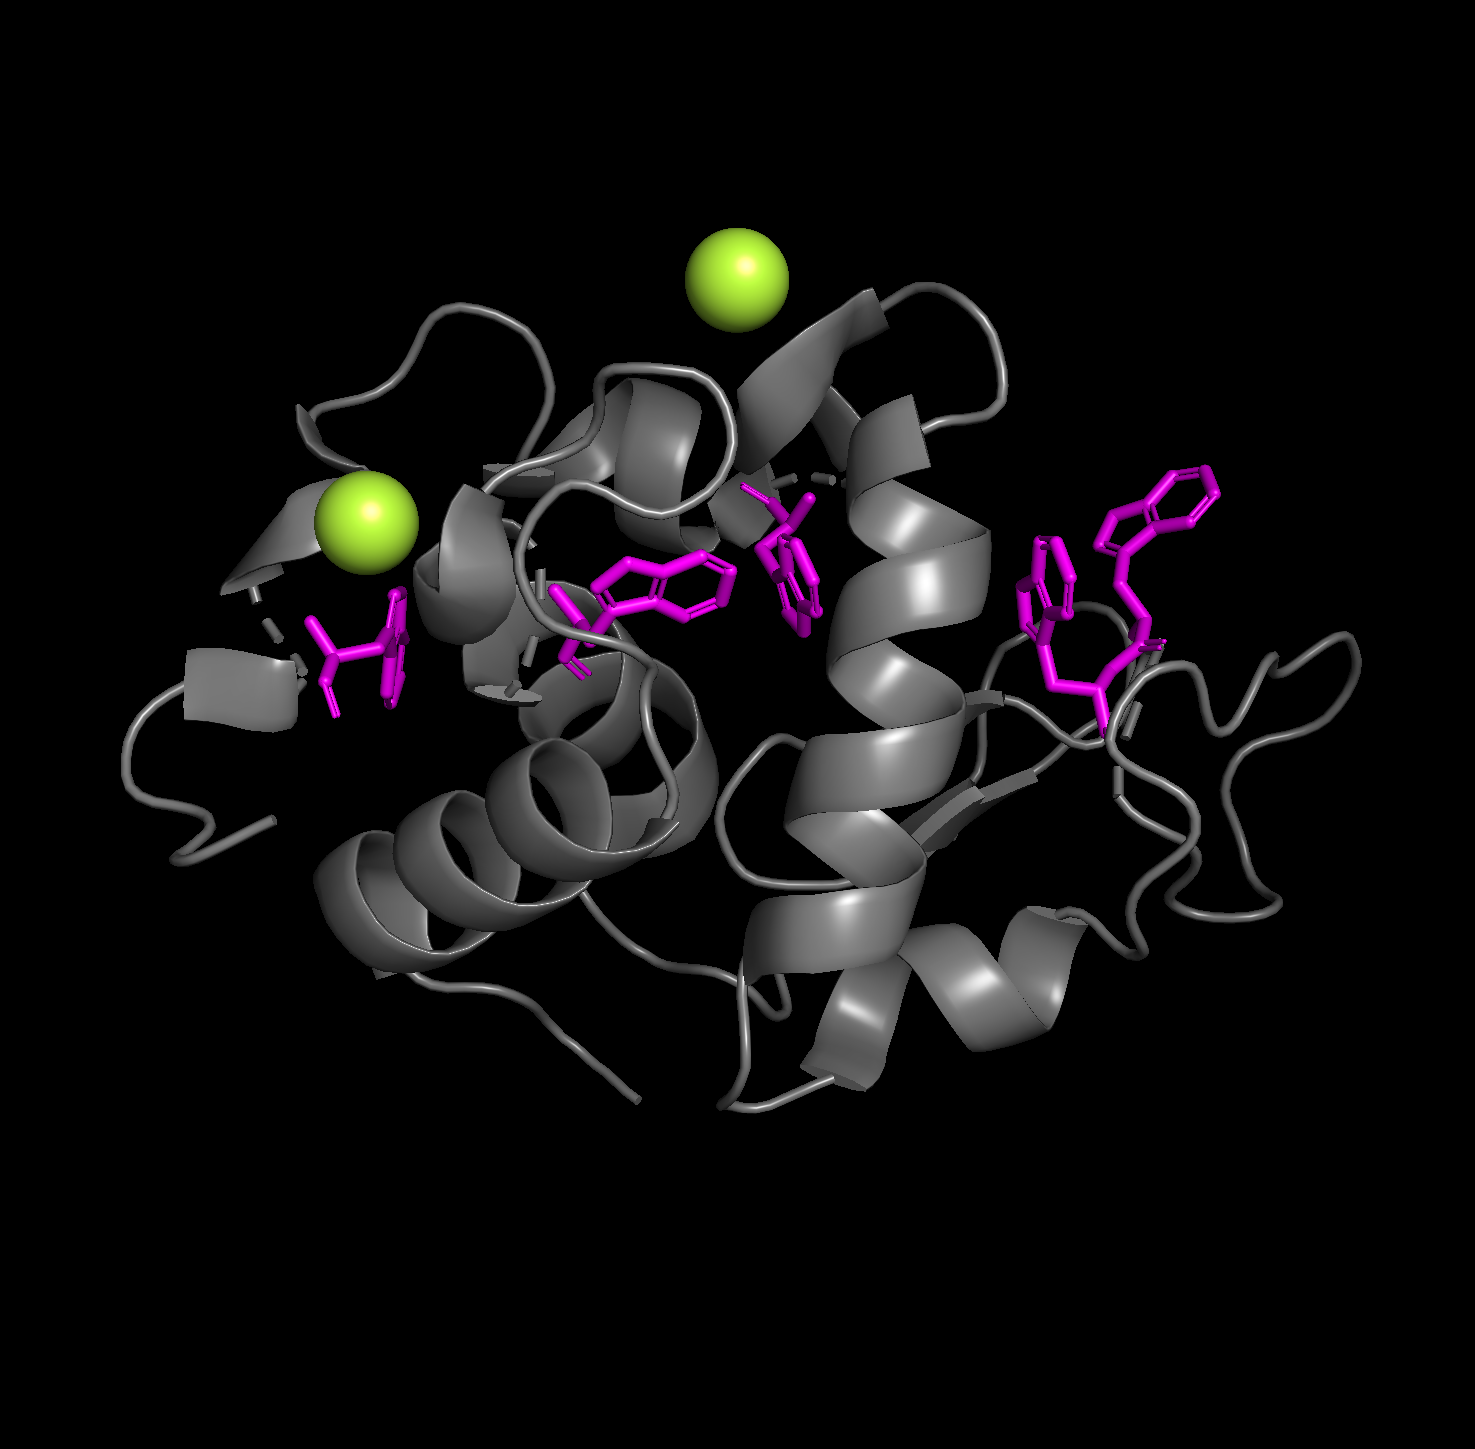
\includegraphics[width=0.5\linewidth]{EggWhiteLysozyme1DPX.png}
    \caption{Pymol view of Egg White Lysozyme with Cl in Green and Tryptophan in Magenta PDB: 1DPX \cite{hilgenfeld_crystallization_2000} } 
\end{figure}



\chapter{Experiment and results}
\label{cha:Experiment}

%Stopped-flow technique and how it enables rapid change of environement

%Description of the apparatus and 

%Wavelength selected and why + a note on the voltage sensitivity of the photomultiplier

%Flushing the apparatus ( from EtOh to H2O to 0 M Guandinum/Unfolding Solution)

% Each MEASUREMENT consisted of: opening,pulling the pistons back, loading sample  in "syringe", mixing, closing, resetting counter, trial run for checking time and intensity, evrything again , real run, plot, fitting and residuals.

%The analysis part consisted in : plotting and fitting.

%the procedure was repeated for different concentrations with a particular attention to flushing when changing between folding/ unfolding solution.

%The chart show the different concentrations and the measured K

%The chevron plot and regression to get k_uf and k_f
A stopped-flow instrument was applied in our experiment (Figure 2.1). This instrument is designed to change the environment of biological particles rapidly by mixing two solutions through a turbulent process. As shown on the left of Figure 2.1, two small syringes, A and B, are filled with solutions and biological particles separately. A large piston rapidly pushes the small syringes, creating turbulence in the chamber (shaded part in the figure).The turbulence will immediately mix the particles and solutions. When the observation particles with several microliters are purged and filled, the flow is abruptly stopped by the stopping syringe, which fills with the waste solution and moves to touch the stop button. \\



\begin{figure}[H]
    \centering
    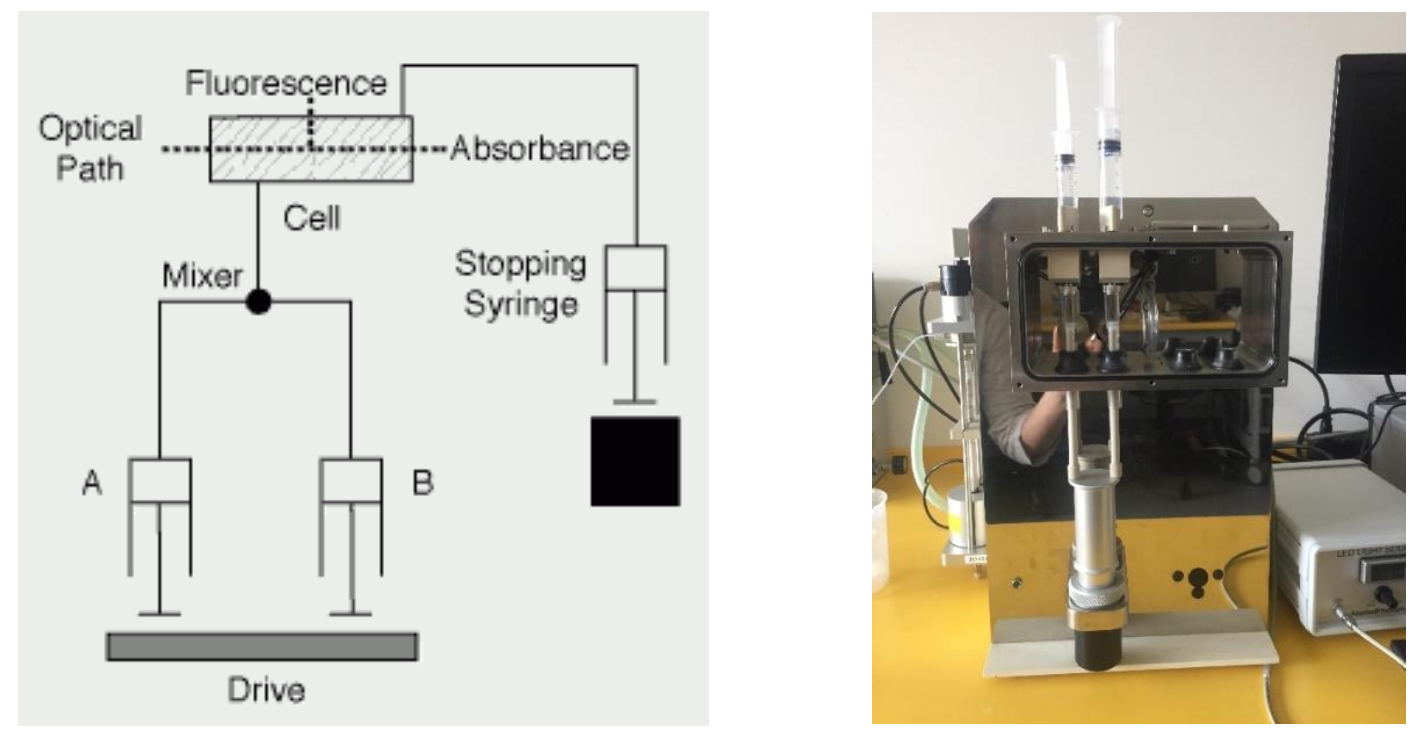
\includegraphics[width = 0.8\textwidth]{Images/stopped-flow instrument.png}
    \caption{The schematic drawing of the stopped-flow instrument(left) and the real instrument we used in the experiment(right)}
    \label{fig:enter-label}
\end{figure}
In our experiment, two large syringes(see right side of Figure 2.1) are attached to the apparatus as the tanks of the solution and biological particle, and a detection unit ( photomultiplier and computer ) is also attached to it. Figure 2.2 shows the redshift on the emission wavelength of the folded and unfolded lysozyme. The detector worked at around 340 to 350 nm to capture the intensity change in fluorescence and distinguish the signal of the folding protein(intensity decreases as the wavelength increases) and the signal of the unfolded protein ( intensity increases as the wavelength increases ).\\

Our stopped-flow apparatus uses syringes in a 5:1 volume ratio, with guanidinium chloride (GdmCl) in the bigger syringe. This setup is designed to achieve the desired final concentration of GdmCl upon mixing with the protein solution.\\

A photomultiplier is used to help us observe the changes in intensity. However, its multiplication ability is not proportional to the voltage .In fact the instrument sensibility does not follow a linear relationship with the Voltage, thus resulting in measured values very quickly getting out of the detection range for minimal changes in Voltage.\\

Solution G contained our protein of interest in 6M GdmCl, ensuring it was in an unfolded state. In contrast, Buffer A contained the same protein in 0M GdmCl, maintaining it in a folded state. These solutions provided the necessary starting points for our folding and unfolding kinetic studies.\\

\begin{figure}[H]
    \centering
    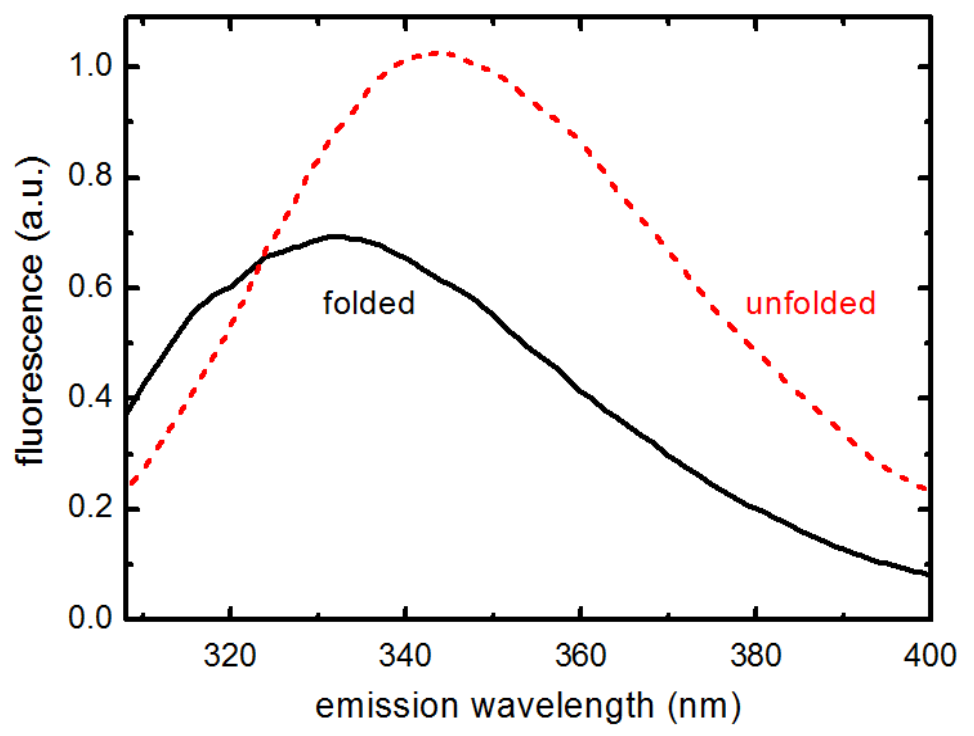
\includegraphics[width = 0.8\textwidth]{Images/RedShift_real.png}
    \caption{Fluorescence spectra for for lysozyme in glycin buffer at pH 2.2 and for unfolded lysozyme in the same buffer with additional 6 M GdmCl. \cite{BiophysicsLabCourse}}
    \label{fig:enter-label}
\end{figure}
The experiment opearations were described in the following steps: 1) open the valves to link the tank syringes to the system. 2) pull the pistons of the syringes to put the remaining liquid back to the tank syringes. 3) remove the tank syringes from the instrument and refill it with the required solutions. 4) put the tank syringes back. 5) pull and push the syringes repeatedly to mix the remaining in the syringes and the new solution. 6) pull the pistons slowly to the bottom to refill the syringes. 7) click the reset in the software, and make several trail runs to find the appropriate time and voltage setting. 8) refill the syringes again and make 5 attempts for each concentration. 9) record the time-intensity curve, take the average of the 5 attempts and apply single exponential fitting. 10) Repeat from 1 until every group is finished.\\

At the beginning of the experiment, the chamber was flushed with ethanol and water to make it a clean environment. Then we used the 0M GmdCl solution, which is actually a buffer(12 mM Glycin*HCl, 0.6 M KCl, pH=2.2) to flush it again for the following experiment. After that, we applied different concentration of GdmCl and lysozyme (See table 2.1), plotted the time-intensity curve and did the single exponential fitting to acquire the apparent rate coefficient($\mathrm{k_{app}}$). The fitted $\mathrm{k_{app}}$ are shown in table 2.1. Theoretically, the chevron plot follows the following equation:
\[
k_{app} = k^0_fe^{\frac{m_f[D]}{RT}} + k^0_{uf}e^{\frac{m_{uf}[D]}{RT}}
\]

\begin{table}[H]
    \centering
    \begin{tabular}{c|c|c|c}
        \textbf{Refolding}\\
        \hline
        2.5 ml syringe &0.5 ml syringe& GdmCl[M]&$k_{app}$[1/s]  \\
        \hline
        0 M GdmCl &6 M GdmCl + 40 $\mathrm{\mu}$M Lysozyme &1.00 &0.158 \\
        \hline
        0.5 M GdmCl &6 M GdmCl + 40 $\mathrm{\mu}$M Lysozyme &1.42 &0.096\\
        \hline
        1.0 M GdmCl &6 M GdmCl + 40 $\mathrm{\mu}$M Lysozyme &1.83 &0.054\\
        \hline
        1.5 M GdmCl &6 M GdmCl + 40 $\mathrm{\mu}$M Lysozyme &2.25 &0.051\\
        \hline
        \textbf{Unfolding}\\
        \hline
        3 M GdmCl &40 $\mathrm{\mu}$M Lysozyme &2.50 & 0.026\\
        \hline
        3.5 M GdmCl &40 $\mathrm{\mu}$M Lysozyme &2.92 &0.028\\
        \hline
        4.0 M GdmCl &40 $\mathrm{\mu}$M Lysozyme &3.33 &0.032\\
        \hline
        4.5 M GdmCl &40 $\mathrm{\mu}$M Lysozyme &3.75 &0.039\\
        \hline
        5 M GdmCl &40 $\mathrm{\mu}$M Lysozyme &4.17 &0.048\\
        \hline
        5.5 M GdmCl &40 $\mathrm{\mu}$M Lysozyme &4.58 &0.062\\
        \hline
        6 M GdmCl &40 $\mathrm{\mu}$M Lysozyme & 5.00&0.082\\
        \hline
    \end{tabular}
    \caption{The results of the experiment}
    \label{tab:my_label}
\end{table}


where $k^0_f$ and $k^0_{uf}$ is the rate coefficient of folding and unfolding, $m_f$ and $m_{uf}$ is the coefficient of the GdmCl concentration change of the folding process and unfolding process. We suppose that the apparent rate is dominated by the folding term while folding, and dominated by unfolding term while unfolding. By taking the logarithm on both side, we can acquire the following equations:
\[
\mathrm{Folding: } ln(k_{app}) = \frac{m_f}{RT}[D] + ln(k_f^0)
\]
\[
\mathrm{Unfolding: } ln(k_{app}) = \frac{m_{uf}}{RT}[D] + ln(k_{uf}^0)
\]

\begin{figure}[H]
    \centering
    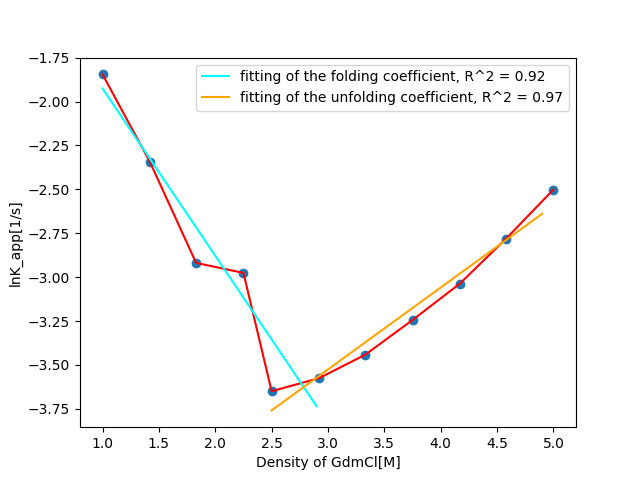
\includegraphics[width = 0.9\textwidth]{Images/Chevronplot.png}
    \caption{Caption}
    \label{fig:enter-label}
\end{figure}
With the linear regression(the cyan line and the orange line in figure 2.3) of the chevron curve in folding and unfolding part, and assuming the temperature is 300K, we acquired the following values:
\[
k_f^0 = 0.378 s^{-1}
\]
\[
k_{uf}^0 = 0.007 s^{-1}
\]
\[
m_f = -2.375 kJ/M
\]
\[
m_{uf} = 1.163 kJ/M 
\]
The equilibrium constant $k_{eq} = \frac{k_f^0}{k_{uf}^0} = 54$, and the Unfolding free energy $\Delta G_{uf}^0 = RTln(k_{eq}) \approx 9.941 kJ/M$.
\begin{comment}

Calculated Molar:
REFolding: 1: 1, 2: 1.42, 3: 1.83, 4: 2.25 

Unfolding: 1: 2.5, 2:2.92, 3: 3.33, 4: 3.75, 5: 4.17, 6: 4.58, 7: 5.00

result of the refolding : k_rf = 0.378
unfolding: k_uf = 0.007
\end{comment}

\chapter{Discussion}
\label{cha:Discussion}
% COMPARE the data with the published paper.
% The published paper focused more on a 3 component system and for this reason we can compare only some values 
%24.22

%The instability of the data due to inabundunt mixing
During the experiment, we did five intensity-time plots for each GdmCl concentration. However, in several plots(0.5, 1.0, 1.5 M GdmCl, Figure 4.2, 4.3, and 4.4), we acquired some weird curves. Theoretically, the plots should be similar if all the parameters(concentration, temperature, voltage) remained the same. But in our experiment, we acquired some apparent non-exponential curves (e.g. 4.2 plot 0) and some curves which have decayed differently with other plots(e.g. 4.2 plot 1). After we increased the mixing times, this problem vanished. This situation indicated that insufficient mixing could be the reason. We speculate that the insufficient mixing will lead to a non-uniform concentration environment for the protein, which means the folding rate of the proteins in the solution could be different. The lysozyme in these different proteins will have a different fluorescence intensity and a different intensity-time curve, which could be the reason for recording a non-fluent curve and curve with different decay rates in our experiment.\\
%temperature is not stabilized and this could induce error in the regression

From the folding and unfolding formula shown in the results part, we will notice that the $\mathrm{lnK_{app}}$ is not only proportional to the concentration of the solution, it is also proportional to the 1/T. So a fixed temperature is expected in the experiment, otherwise it's not reasonable to do a linear fitting between GdmCl concentration and the apparent rate. However, in our experiment, the temperature of the system is not perfectly the same. It is fluctuating between $29^\circ $C to $30^\circ $C. A rough estimate of the influence of $1^\circ$C change is that it will result in $\frac{1}{300}$ change in $\mathrm{m_f}$ or $\mathrm{m_{uf}}$. Since it's relatively small, we could omit the influence of temperature fluctuation in our experiment. However, it is very important to keep a stable temperature during the experiment with this experiment designation.\\

We can better understand the results shown in Figure 2.3 by comparing the published\cite{sasahara} data. In this paper, the $m_{uf}$ under pH 2.2 is 10.57 kJ/M, which is 10 times larger than our data. The different temperatures (298K and 303K)between there and our experiment could be one reason. Besides, they have many more measurements(around twenty) on this branch, while we just have seven. The $k_f^0$ = 0.78/s, $k_{uf}^0 = 3.55 \times 10^{-4}$/s by on-pathway model. These two values have the same order of magnitude as our fitting results. However, this result is from a three-state model(with folding, unfolding, and intermediate state, instead of just folding and unfolding state). In the paper, they built several three-state models, which brings more convincing results. \\

%Real protein folding has more than two states, there could be some intermediate state in the system, which makes it just a rough estimation

Protein folding is a complex process that often involves more than just two states, the fully folded and fully unfolded forms. Intermediate states can exist within the system, complicating the analysis and interpretation of folding kinetics. These intermediates can represent partially folded structures or transient conformations. Our experiment assumes a simple two-state model for practical reasons, but we acknowledge that this is a rough estimation and that the actual folding pathway may involve multiple intermediates. This simplification can lead to inaccuracies in our calculations, but it provides a workable framework for generating initial insights into the folding process.\\

% The following plot assumes that the Lysozime is a 2-state folder protein, with 1 array when completely unfolded and 1 state when completely folded, we know that this is not the case for several reasons( e.g Publication/ common sense) but  we assumed it to be true to simply the calculation of a Chevron Plot.

The Chevron plot assumes that lysozyme behaves as a two-state folder, with one state when completely unfolded and another when completely folded. Although we recognize that lysozyme may not strictly follow this two-state model, as supported by literature\cite{sasahara}and common knowledge, this assumption simplifies our calculations. Intermediate states and deviations from the two-state model are acknowledged, but for the purposes of this experiment, the two-state model provides a useful framework for analyzing the folding kinetics and generating the Chevron plot. Future studies could refine this model by incorporating intermediate states and more complex folding pathways.\\

%6M solution is oversaturated, the real concentration might be lower than 6M, for this reason al the solutions could be systematically shifted towards lower concentrations

Guanidinium chloride at 6M is already in the oversaturation region of Guanidinium water solubility, meaning that the actual concentration might be lower than 6M. This discrepancy could systematically shift all our solutions towards lower concentrations than intended.
This systematic shift  could be accounted in the experimental process just by measuring the density of the resulting solution and using that value instead of the assumed 6M.\\

%discuss cherry picking of traces for when plotting the chevron plot, the reason why we exclude decay function is when they are over the sensibility range of the Photo Multiplier Tube,  

When selecting the traces for which we would fit, we had to exclude certain decay traces that exceeded the sensitivity range we set for the photomultiplier tube (PMT) and also set specific ranges where the traces looked consistent.
We also fitted an exponential decay function only to the traces that looked like good traces.\\
This process could be interpreted as cherry picking of only the expected results. For this reason we provide all traces recorded in the appendix with a note on the traces and ranges used for the fitting.\\

We had to exclude many of the recorded traces because of issues with our experimental approach described above regarding insufficient mixing.
This is highlighted by the fact that with the Unfolding Solutions, we provided enough mixing in the reservoir to create a consistent concentration, and the resulting traces were perfect and we didn´t need to manually select any traces.\\



The chambers used in the stopped-flow apparatus were washed thoroughly, especially when making significant changes in the molar concentration of GdmCl or when switching protein solutions. This cleaning ensures that the observed fluorescence changes are due solely to the protein of interest and not residual substances from previous experiments.\\
% Careful load of the syringes is required to avoid bubbles in order to avoid any fluorescence artifact

Careful loading of syringes is essential to avoid introducing air bubbles, which can cause fluorescence artifacts, thus a final slow and steady charging of the syringes from the reservoirs is done after thorough mixing.\\
%The Chambers were washed very toroughly when doing big changes in molar concetration of Guanidinium Chloride or changing protein solution



%A trial run with each solution was performed each time before every measurement, this was considered priming and allowed us to check beforehand for any adjustments in intensity or time recorded.

Before each measurement, we conducted a trial run with each solution. This priming step allowed us to adjust the intensity settings and ensure that the time range recorded the full exponential decay curve
. These trial runs are crucial for verifying that the system is correctly set up and that the solutions are properly mixed and at the intended concentrations.\\




\begin{comment}
    
Fitting the mean of multiple functions yields a lower fitting error compared to fitting multiple traces individually. This approach is statistically incorrect and can be considered a form of p-hacking. It is only valid if the mean of the individual fits is identical, meaning that the standard error of the fit on the resulting function equals the mean of the standard errors of the individual fits.\\
Since we did not verify this condition and assumed the equality based on the traces describing the same event, this method does not represent the proper way to conduct experimental work. In experimental science, it is crucial to observe and verify assumptions rather than taking them for granted and adjusting data to fit our expectations.
During our experimental work, we assumed that the exponential decay of all traces should be equal, given that they describe the same folding event. However, this assumption was not experimentally verified, which undermines the reliability of our analysis.\\

\end{comment}
The currently accepted model for protein folding is co-translational folding, which emphasizes the complexity of early events in the life of newly synthesized proteins. The ribosome plays a crucial role in coordinating these processes, acting as a platform for the regulated association of enzymes, targeting factors, and chaperones. This co-translational model highlights that protein folding is influenced by the cellular environment and especially the ribosome in a progressive manner \cite{kramer_ribosome_2009} following the addition of new aminoacids to the protein sequence.\\


Given the complexity of co-translational folding\cite{javed_ribosome_2017}, the assumption that an unfolded protein can always refold to its native state upon a pH change is oversimplified and limits the biological significance of the stopped-flow kinetics approach. This method does not fully account for the ribosome's role, the progressivity of folding and the dynamic environment within the cell that influences protein folding. Therefore, while stopped-flow kinetics can provide valuable insights into folding mechanisms, its limitations must be acknowledged, and results should be interpreted with caution regarding their relevance to in vivo conditions.









\printbibliography

\chapter{Appendix}
\label{cha:Appendix}

\begin{figure}[H]
    \centering
    \begin{subfigure}[b]{0.45\textwidth}
        \centering
        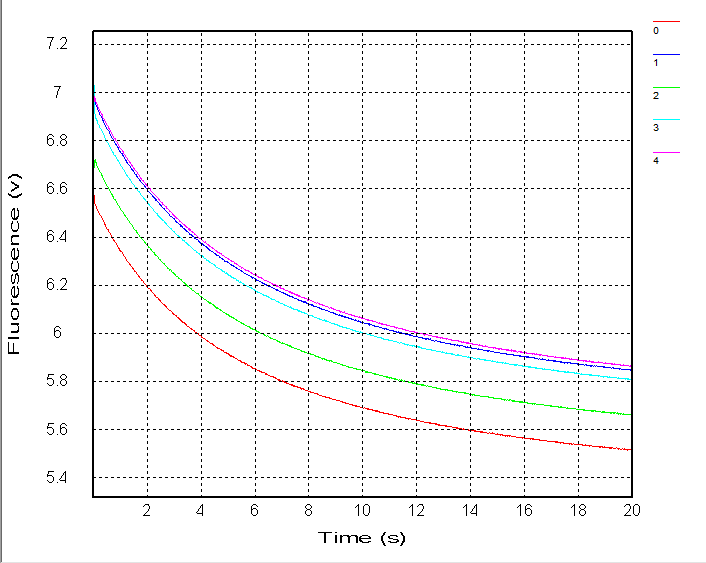
\includegraphics[width=\textwidth]{Images/G8/rf1_raw.PNG}
        \caption{Raw data }
        \label{fig:sub1}
    \end{subfigure}
    \hspace{0cm} % Adjust the horizontal space between subfigures as needed
    \begin{subfigure}[b]{0.45\textwidth}
        \centering
        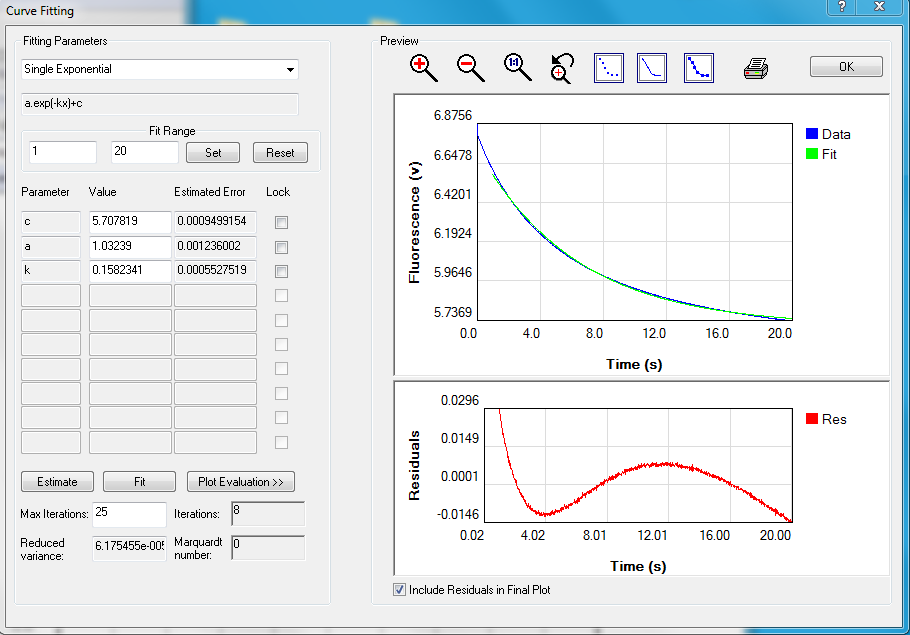
\includegraphics[width=\textwidth]{Images/G8/rf1_fitting.PNG}
        \caption{Fitting}
        \label{fig:sub2}
    \end{subfigure}
    \caption{Refolding at  1.00 M GdmCl }
    \label{fig:main}
\end{figure}
Mean of traces 0,1,2,3,4 used for the fitting for time range 1-20 s.
\begin{figure}[H]
    \centering
    \begin{subfigure}[b]{0.45\textwidth}
        \centering
        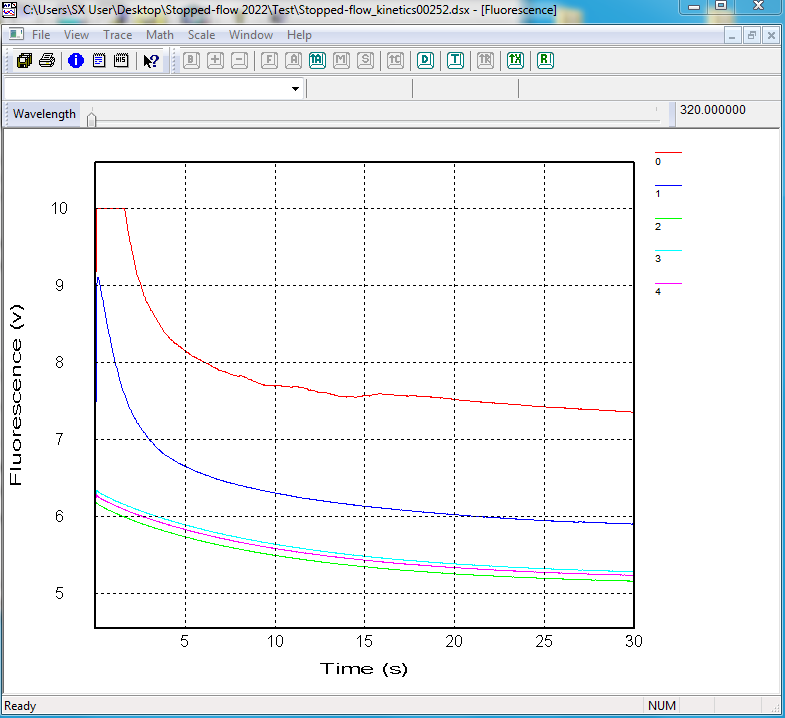
\includegraphics[width=\textwidth]{Images/G8/rf2_raw.PNG}
        \caption{Raw data }
        \label{fig:sub1}
    \end{subfigure}
    \hspace{0cm} % Adjust the horizontal space between subfigures as needed
    \begin{subfigure}[b]{0.45\textwidth}
        \centering
        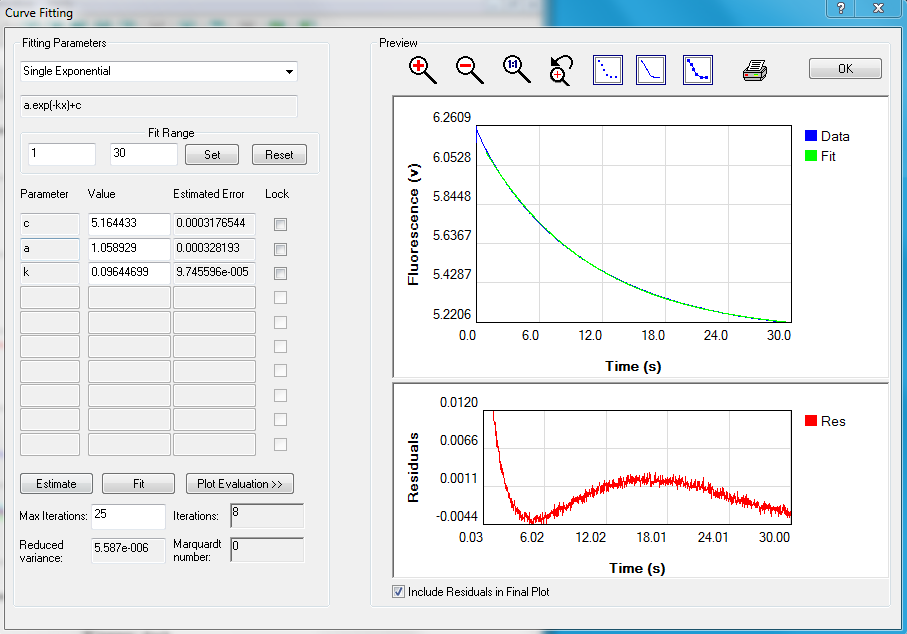
\includegraphics[width=\textwidth]{Images/G8/rf2_fitting.PNG}
        \caption{Fitting}
        \label{fig:sub2}
    \end{subfigure}
    \caption{Refolding at  1.42 M GdmCl }
    \label{fig:main}
\end{figure}
Mean of traces 2,3,4 used for the fitting for time range 1-30 s.
\begin{figure}[H]
    \centering
    \begin{subfigure}[b]{0.45\textwidth}
        \centering
        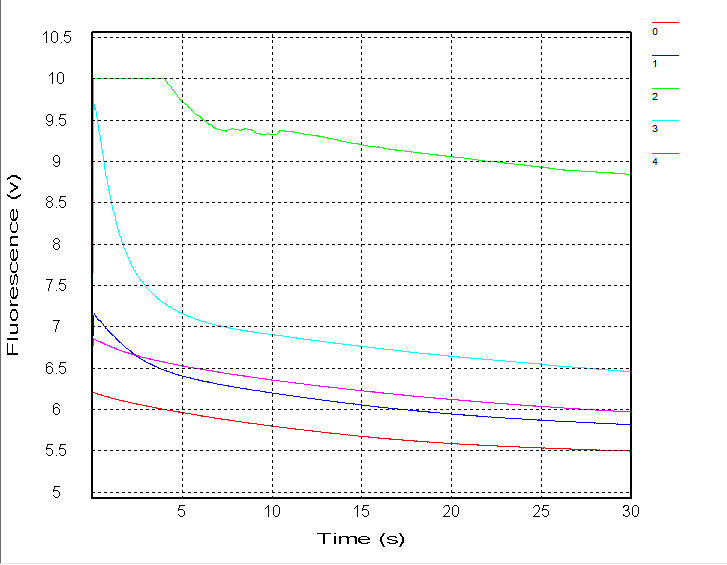
\includegraphics[width=\textwidth]{Images/G8/rf3-raw.PNG}
        \caption{Raw data }
        \label{fig:sub1}
    \end{subfigure}
    \hspace{0cm} % Adjust the horizontal space between subfigures as needed
    \begin{subfigure}[b]{0.45\textwidth}
        \centering
        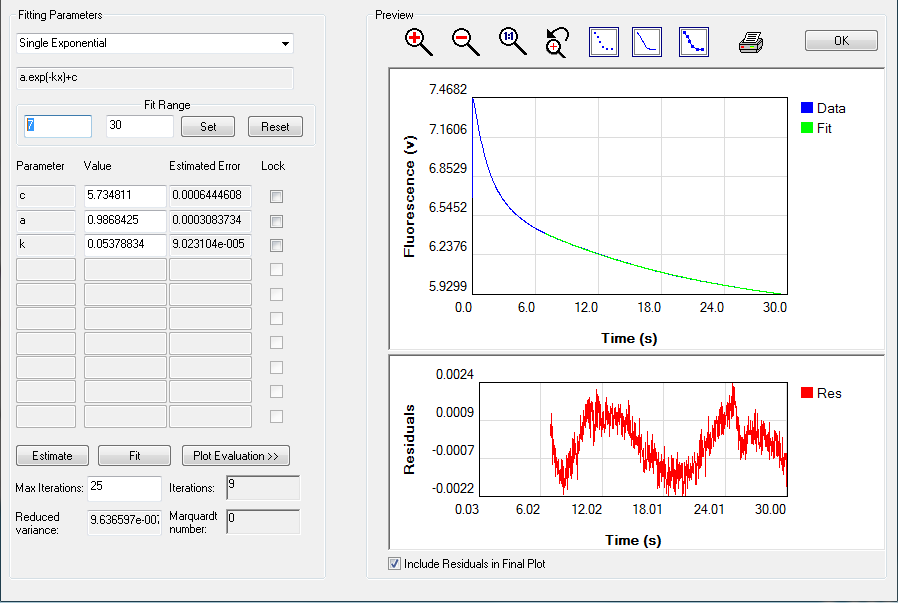
\includegraphics[width=\textwidth]{Images/G8/rf3_fitting.PNG}
        \caption{Fitting}
        \label{fig:sub2}
    \end{subfigure}
    \caption{Refolding at  1.83 M GdmCl }
    \label{fig:main}
\end{figure}
Mean of traces 0,1,3,4 used for the fitting for time range 7-30 s.
\begin{figure}[H]
    \centering
    \begin{subfigure}[b]{0.45\textwidth}
        \centering
        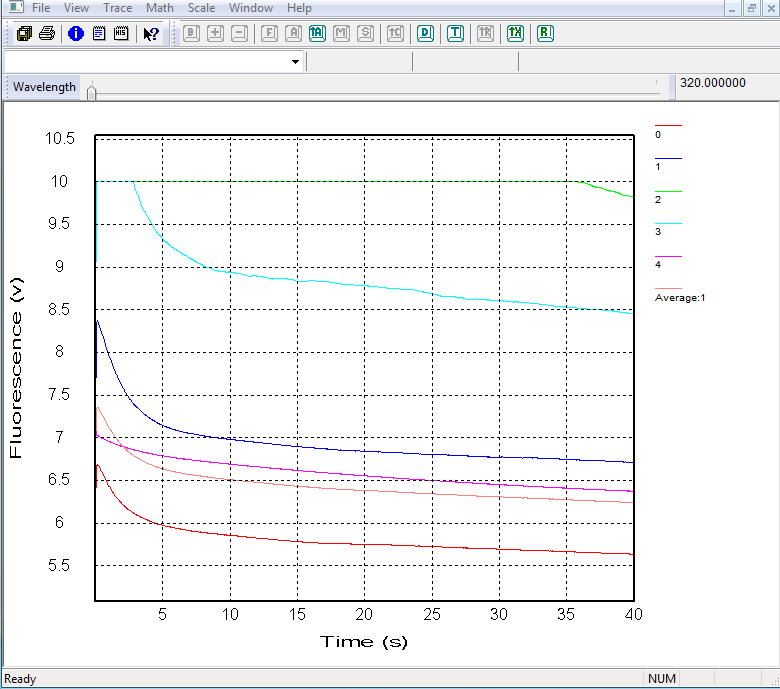
\includegraphics[width=\textwidth]{Images/G8/rf4_raw.PNG}
        \caption{Raw data }
        \label{fig:sub1}
    \end{subfigure}
    \hspace{0cm} % Adjust the horizontal space between subfigures as needed
    \begin{subfigure}[b]{0.45\textwidth}
        \centering
        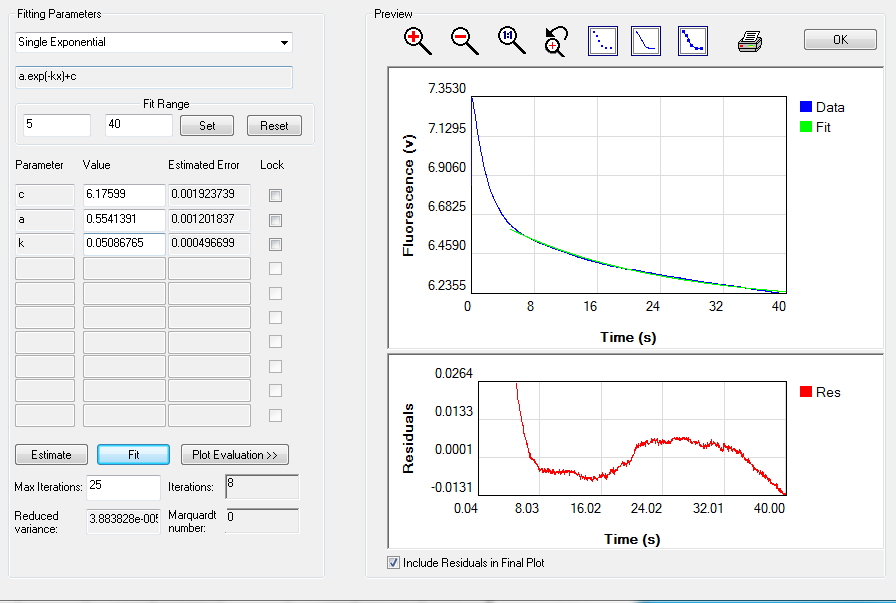
\includegraphics[width=\textwidth]{Images/G8/rf4_fitting.PNG}
        \caption{Fitting}
        \label{fig:sub2}
    \end{subfigure}
    \caption{Refolding at  1.25 M GdmCl }
    \label{fig:main}
\end{figure}
Mean of traces 0,1,4 used for the fitting for time range 5-40 s.
\begin{figure}[H]
    \centering
    \begin{subfigure}[b]{0.45\textwidth}
        \centering
        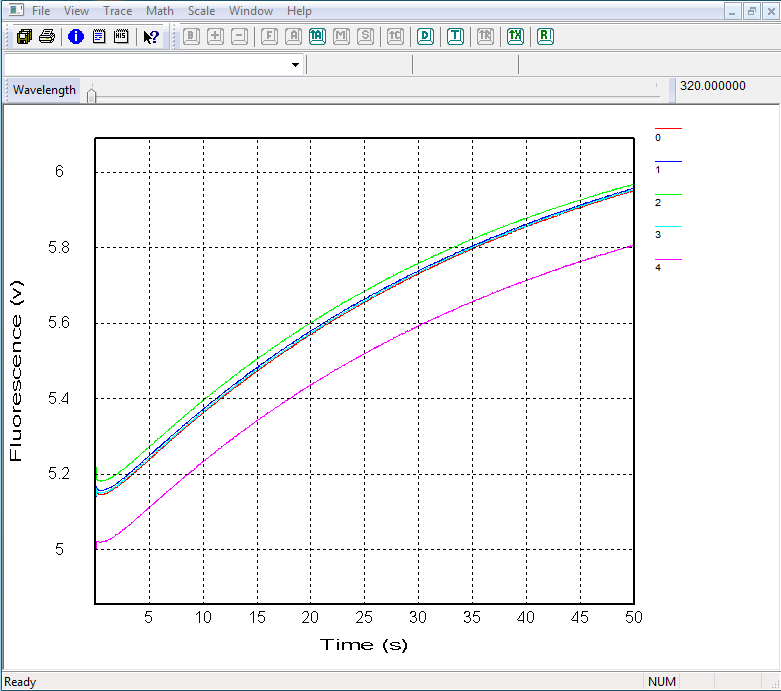
\includegraphics[width=\textwidth]{Images/G8/uf1_raw.PNG}
        \caption{Raw data }
        \label{fig:sub1}
    \end{subfigure}
    \hspace{0cm} % Adjust the horizontal space between subfigures as needed
    \begin{subfigure}[b]{0.45\textwidth}
        \centering
        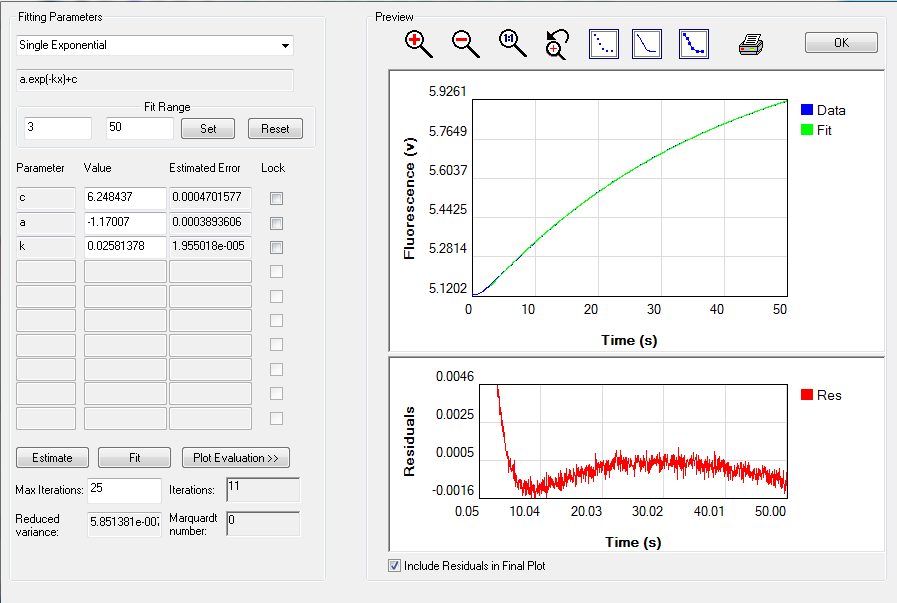
\includegraphics[width=\textwidth]{Images/G8/uf1_fitting.PNG}
        \caption{Fitting}
        \label{fig:sub2}
    \end{subfigure}
    \caption{Unfolding at 2.50 M GdmCl }
    \label{fig:main}
\end{figure}
Mean of traces 0,1,2,3,4 used for the fitting for time range 3-50 s.
\begin{figure}[H]
    \centering
    \begin{subfigure}[b]{0.45\textwidth}
        \centering
        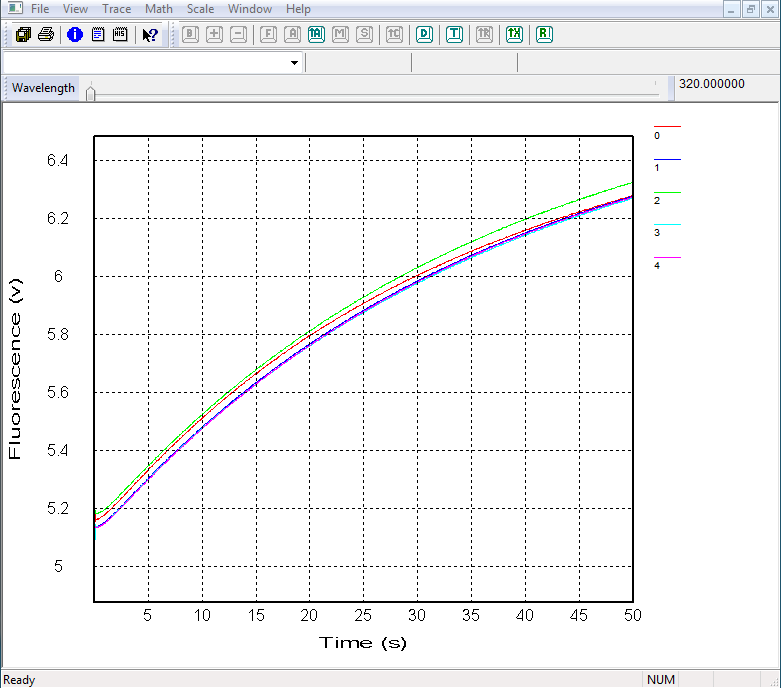
\includegraphics[width=\textwidth]{Images/G8/uf2_raw.PNG}
        \caption{Raw data }
        \label{fig:sub1}
    \end{subfigure}
    \hspace{0cm} % Adjust the horizontal space between subfigures as needed
    \begin{subfigure}[b]{0.45\textwidth}
        \centering
        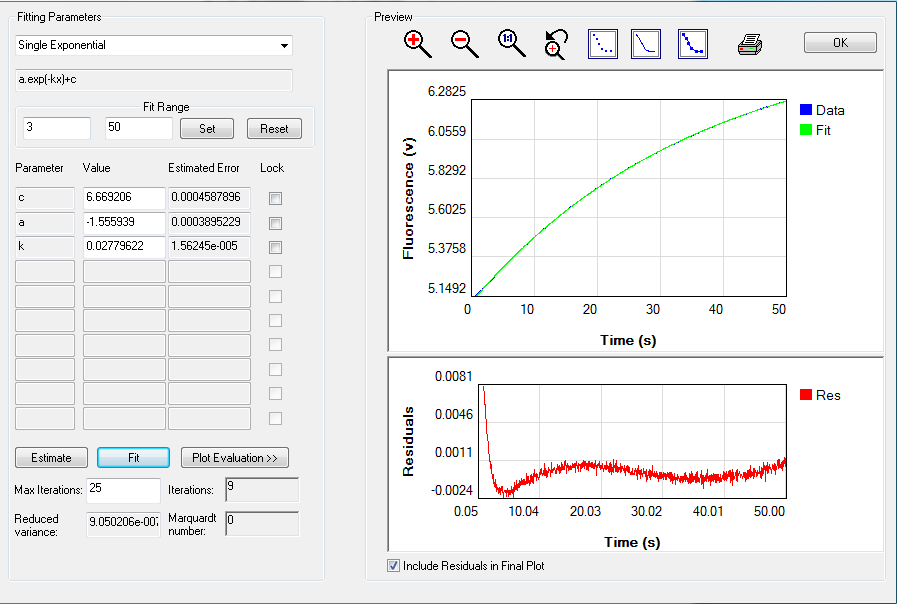
\includegraphics[width=\textwidth]{Images/G8/uf2_fitting.PNG}
        \caption{Fitting}
        \label{fig:sub2}
    \end{subfigure}
    \caption{Unfolding at 2.92 M GdmCl }
    \label{fig:main}
\end{figure}
Mean of traces 0,1,2,3,4 used for the fitting for time range 3-50 s.
\begin{figure}[H]
    \centering
    \begin{subfigure}[b]{0.45\textwidth}
        \centering
        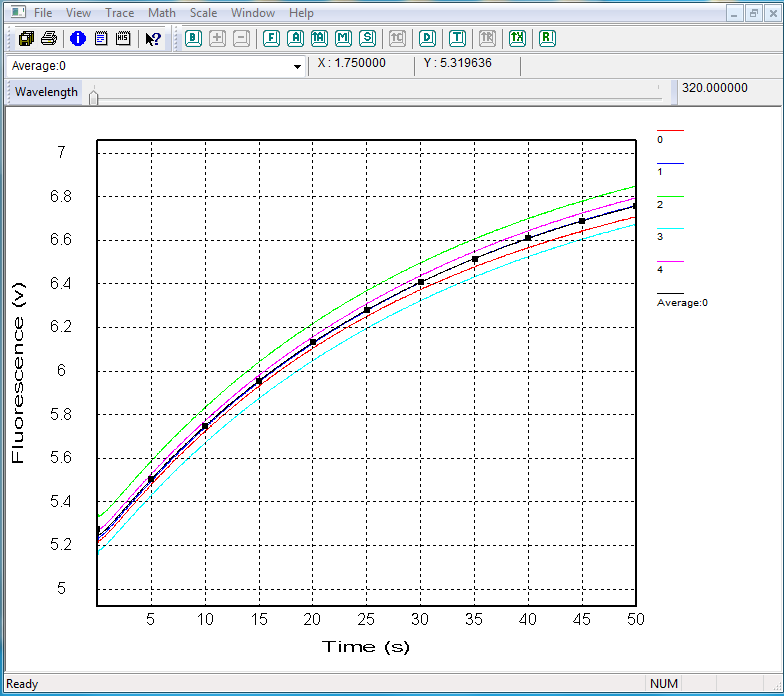
\includegraphics[width=\textwidth]{Images/G8/uf3_raw.PNG}
        \caption{Raw data }
        \label{fig:sub1}
    \end{subfigure}
    \hspace{0cm} % Adjust the horizontal space between subfigures as needed
    \begin{subfigure}[b]{0.45\textwidth}
        \centering
        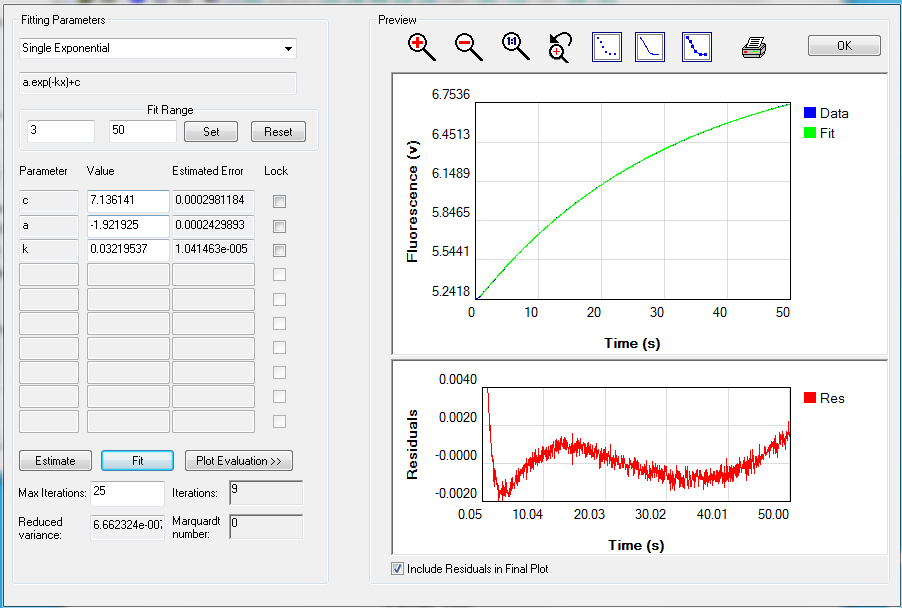
\includegraphics[width=\textwidth]{Images/G8/uf3_fitting.PNG}
        \caption{Fitting}
        \label{fig:sub2}
    \end{subfigure}
    \caption{Unfolding at 3.33 M GdmCl }
    \label{fig:main}
\end{figure}
Mean of traces 0,1,2,3,4 used for the fitting for time range 3-50 s.
\begin{figure}[H]
    \centering
    \begin{subfigure}[b]{0.45\textwidth}
        \centering
        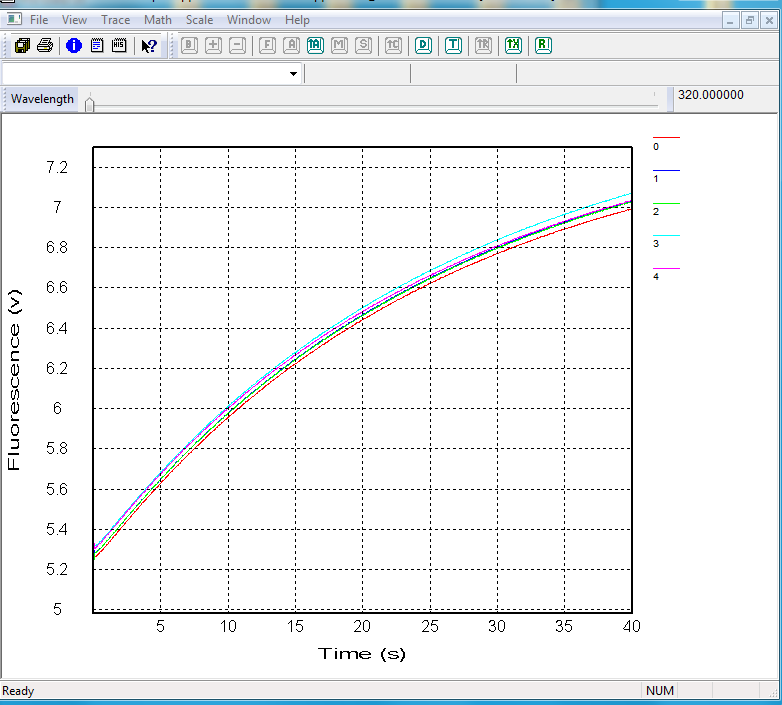
\includegraphics[width=\textwidth]{Images/G8/uf4_raw.PNG}
        \caption{Raw data }
        \label{fig:sub1}
    \end{subfigure}
    \hspace{0cm} % Adjust the horizontal space between subfigures as needed
    \begin{subfigure}[b]{0.45\textwidth}
        \centering
        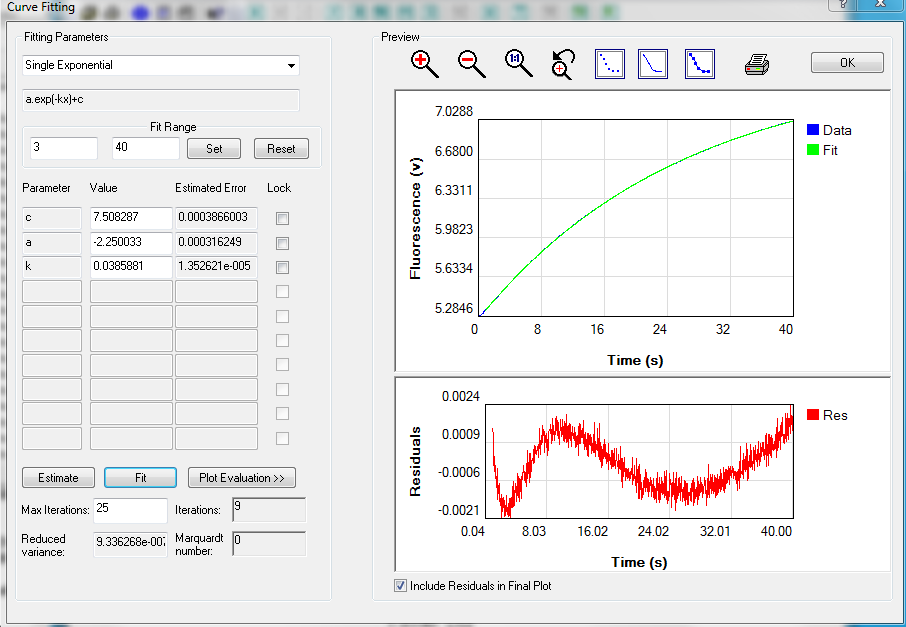
\includegraphics[width=\textwidth]{Images/G8/uf4_fitting.PNG}
        \caption{Fitting}
        \label{fig:sub2}
    \end{subfigure}
    \caption{Unfolding at 3.75 M GdmCl }
    \label{fig:main}
\end{figure}
Mean of traces 0,1,2,3,4 used for the fitting for time range 3-40 s.
\begin{figure}[H]
    \centering
    \begin{subfigure}[b]{0.45\textwidth}
        \centering
        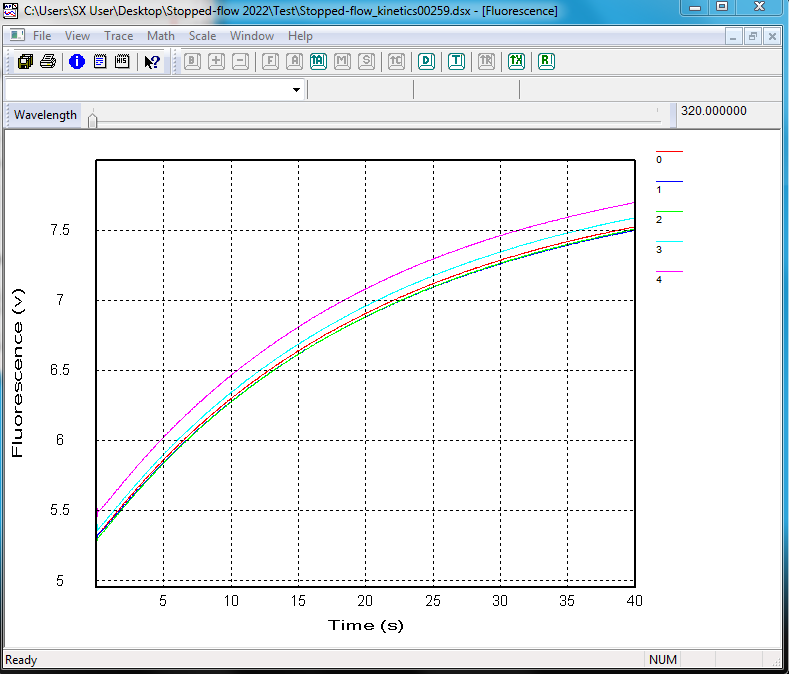
\includegraphics[width=\textwidth]{Images/G8/uf5_raw.PNG}
        \caption{Raw data }
        \label{fig:sub1}
    \end{subfigure}
    \hspace{0cm} % Adjust the horizontal space between subfigures as needed
    \begin{subfigure}[b]{0.45\textwidth}
        \centering
        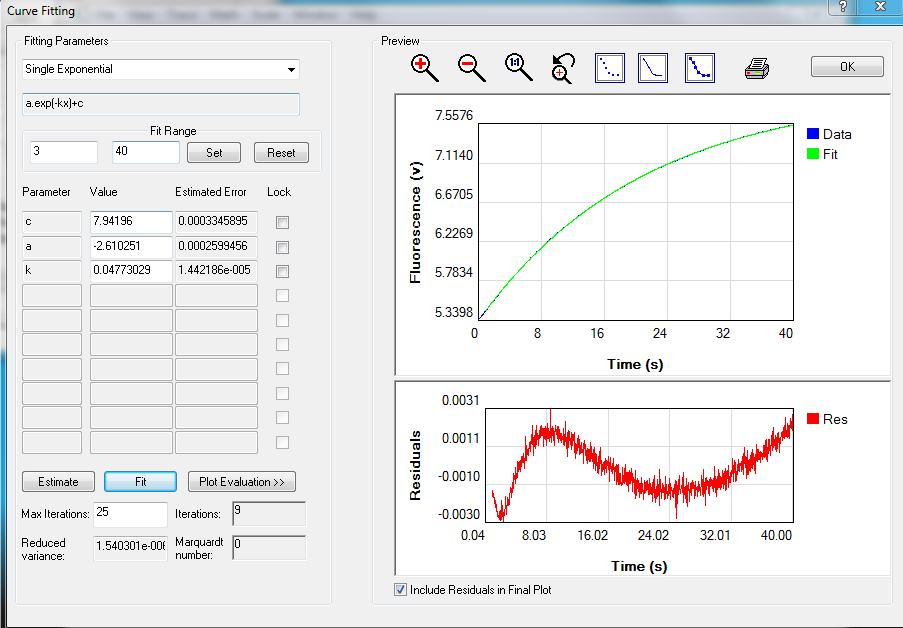
\includegraphics[width=\textwidth]{Images/G8/uf5_fitting.PNG}
        \caption{Fitting}
        \label{fig:sub2}
    \end{subfigure}
    \caption{Unfolding at 4.17 M GdmCl }
    \label{fig:main}
\end{figure}
Mean of traces 0,1,2,3,4 used for the fitting for time range 3-40 s.
\begin{figure}[H]
    \centering
    \begin{subfigure}[b]{0.45\textwidth}
        \centering
        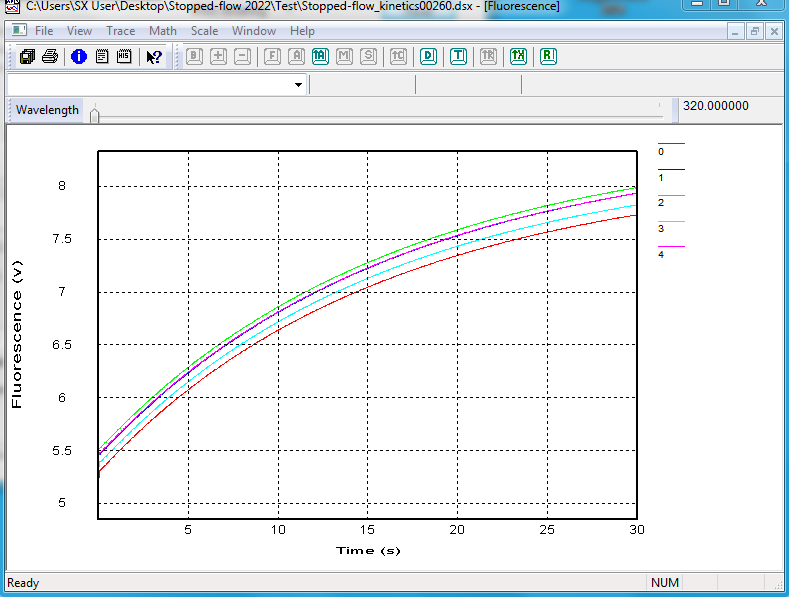
\includegraphics[width=\textwidth]{Images/G8/uf6_raw.PNG}
        \caption{Raw data }
        \label{fig:sub1}
    \end{subfigure}
    \hspace{0cm} % Adjust the horizontal space between subfigures as needed
    \begin{subfigure}[b]{0.45\textwidth}
        \centering
        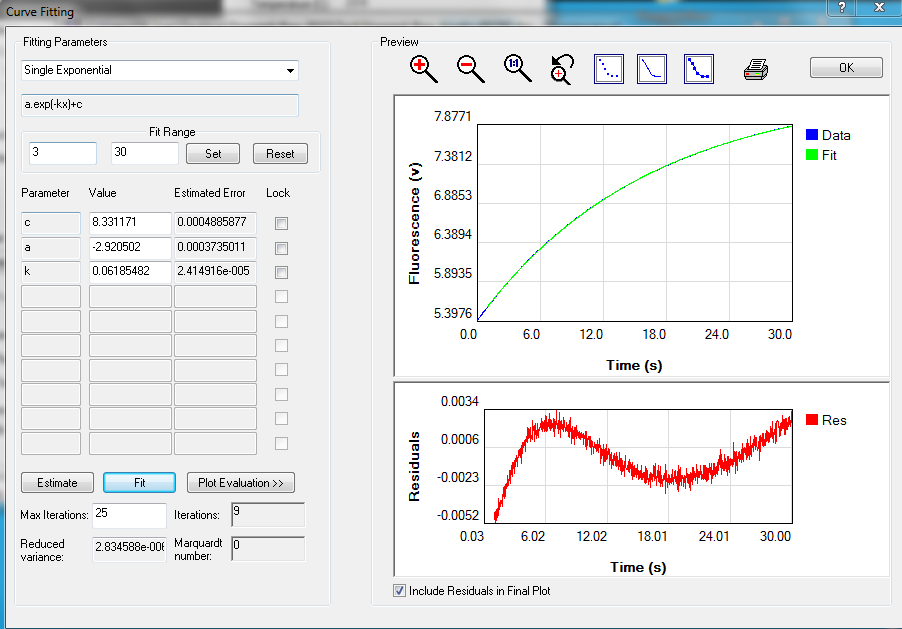
\includegraphics[width=\textwidth]{Images/G8/uf6_fitting.PNG}
        \caption{Fitting}
        \label{fig:sub2}
    \end{subfigure}
    \caption{Unfolding at 4,58 M GdmCl }
    \label{fig:main}
\end{figure}
Mean of traces 0,1,2,3,4 used for the fitting for time range 3-30 s.
\begin{figure}[H]
    \centering
    \begin{subfigure}[b]{0.45\textwidth}
        \centering
        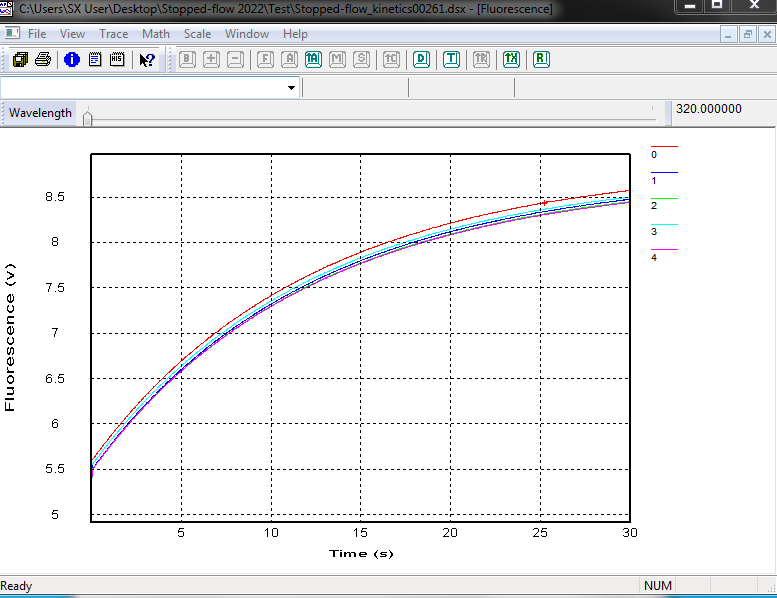
\includegraphics[width=\textwidth]{Images/G8/uf7_raw.PNG}
        \caption{Raw data }
        \label{fig:sub1}
    \end{subfigure}
    \hspace{0cm} % Adjust the horizontal space between subfigures as needed
    \begin{subfigure}[b]{0.45\textwidth}
        \centering
        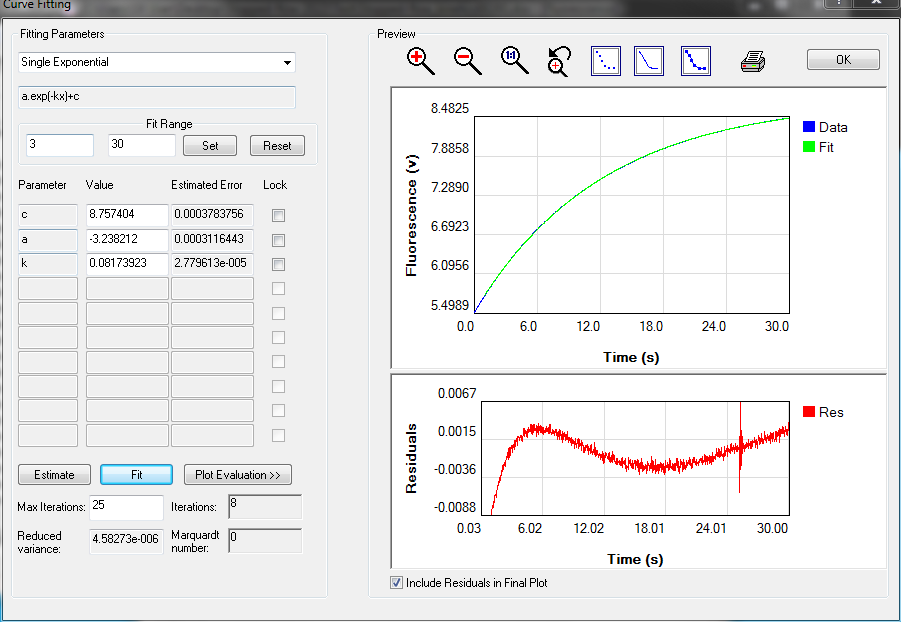
\includegraphics[width=\textwidth]{Images/G8/uf7_fitting.PNG}
        \caption{Fitting}
        \label{fig:sub2}
    \end{subfigure}
    \caption{Unfolding at 5.00 M GdmCl }
    \label{fig:main}
\end{figure}
Mean of traces 0,1,2,3,4 used for the fitting for time range 3-30 s.

% The fitting error for the mean of multiple functions is lower than the fitting error of multiple traces fitted one by one, the method we used is statistically incorrect and actually considered to be a form of p-hacking.
% Only in one case this is an acceptable way of proceeding in the calculation, it is only when we know that the mean of the individual fits are all the same we can say that the std. error of the fit on the resulting function equal to the mean of the functions is equal to the mean of std. errors ( meaning only if : std.error( mean(fit(func.1) + fit(func.2) + fit(func.3)) == std.error( fit (mean( func.1 + func.2 + func.3) ) 

% Considering that we didn´t actually verify this condition before the calculation but just assumed that since they all describe the same event, their exp. decay should all be equal this doesn´t represent the proper way to proceed when doing experimental work, during experimental work we "OBSERVE" and "CHECK" if our assumptions hold true instead of taking the assumptions for granted and looking for what data fits our idea. 

\end{document}